\chapter{Đọc thêm 3: Mối liên hệ giữa Tiền mã hóa và Sự chú ý trên Google Trends (Aslanidis, Bariviera \& López)}
\label{ch:M4L2DT3}

% Nguồn: Aslanidis, N., Bariviera, A. F., & López, Ó. G. ``The link between cryptocurrencies and Google Trends attention.'' Finance Research Letters, 47, 2022.
% Phần cần đọc: Toàn bộ bài báo
% Nội dung bắt buộc đọc: được kiểm tra trong mọi bài đánh giá (kể cả Quiz).

\section{Thông tin nguồn}

\begin{itemize}
  \item \textbf{Nguồn:} Aslanidis, Nektarios, Aurelio F. Bariviera, and Óscar G. López. \emph{The link between cryptocurrencies and Google Trends attention}. Finance Research Letters, 47, 2022. \url{https://doi.org/10.1016/j.frl.2021.102654}
  \item \textbf{Phần cần đọc:} Toàn bộ nội dung
\end{itemize}

\section{Tóm tắt}

Bài báo này xem xét lại mối liên hệ giữa tiền mã hóa và sở thích được bộc lộ công khai của công chúng, được đo lường gián tiếp thông qua các lượt tìm kiếm trực tuyến. Chúng tôi cho thấy rằng tiền mã hóa không liên quan đến một chỉ số bất định chung như được đo bằng dữ liệu Google Trends của Castelnuovo and Tran (2017). Thay vào đó, tiền mã hóa gắn liền với một thước đo sự chú ý (tìm kiếm) trên Google Trends đặc thù cho thị trường này. Cụ thể, chúng tôi phát hiện một luồng thông tin hai chiều giữa sự chú ý trên Google Trends và lợi suất tiền mã hóa kéo dài đến sáu ngày. Ngoài ra, luồng thông tin từ độ biến động của tiền mã hóa đến sự chú ý trên Google Trends dường như lớn hơn so với chiều ngược lại. Cuối cùng, chúng tôi ghi nhận một sự phụ thuộc đuôi (tail dependence) đáng kể giữa lợi suất tiền mã hóa và Google Trends. Các mối quan hệ này đều đúng đối với năm loại tiền mã hóa được phân tích và các cách kết hợp khác nhau của chỉ số Google Trends Cryptocurrency được đề xuất.

\begin{itemize}
  \item \textbf{Phân loại JEL:} C4, G01, G14
  \item \textbf{Từ khóa:} Tiền mã hóa, Google Trends, Entropy chuyển giao (transfer entropy), Sự chú ý thị trường
\end{itemize}

\section{1. Giới thiệu}

Kể từ khi ra đời năm 2009, Bitcoin đã ngày càng thu hút sự chú ý của các nhà đầu tư, nhà nghiên cứu, tổ chức tài chính và nhà hoạch định chính sách. Những người ủng hộ Bitcoin đầu tiên là những người theo chủ nghĩa tự do cá nhân và những tín đồ thực thụ của tiền mã hóa, những người chỉ trích cuộc khủng hoảng tài chính toàn cầu 2008--2009. Các nhà đầu tư này xem blockchain như một cơ chế để vượt qua hệ thống tài chính truyền thống, vốn bị chỉ trích nặng nề vì quy định lỏng lẻo đã dẫn đến cuộc khủng hoảng nói trên (Karlstrøm, 2014; Dallyn, 2017). Làn sóng thứ hai của những người đam mê Bitcoin là các nhà đầu cơ, những người nhìn thấy ở Bitcoin (và các đồng tiền mã hóa mới phát hành) cơ hội đầu tư với lợi suất cao (Bouoiyour et al., 2015). Làn sóng thứ ba của những người tham gia thị trường là các tổ chức tài chính, vốn muốn đưa công nghệ blockchain vào ngành của mình và cung cấp cho nhà đầu tư các nền tảng đầu tư an toàn hơn (Guo and Liang, 2016; Patki and Sople, 2020). Đồng thời, các chính phủ bắt đầu lo ngại về những tác động tiêu cực tiềm ẩn của tiền mã hóa. Nhiều quốc gia đã ban hành các quy định (ví dụ như luật thuế, luật chống rửa tiền/chống tài trợ khủng bố; xem Global Legal Research Center (2018)) và đưa ra cảnh báo về mức độ rủi ro cao của loại hình đầu tư này (Martin, 2021). Cuối cùng, làn sóng thứ tư của những người tham gia thị trường tiền mã hóa hiện nay liên quan đến các ngân hàng trung ương và các đồng tiền kỹ thuật số của ngân hàng trung ương (Central Bank Digital Currencies) (Fernández-Villaverde et al., 2020; Wang et al., 2021a). Để có một tổng quan chi tiết về sự phát triển và hiện trạng nghiên cứu về tiền mã hóa, chúng tôi giới thiệu độc giả tham khảo Corbet et al. (2019), Bariviera and Merediz-Solà (2021), cùng nhiều nghiên cứu khác.

Đồng thời, quá trình số hóa ngày càng sâu rộng của nền kinh tế đã để lại một dấu vết số mà, theo một cách nào đó, bộc lộ sở thích, thị hiếu hoặc thói quen tiêu dùng. Google Trends đã được chứng minh là hữu ích cho việc dự báo hiện tại (nowcasting) và dự báo các chỉ số kinh tế (Vicente et al., 2015) cũng như dự đoán kết quả chính trị (Mavragani and Tsagarakis, 2016). Vì tiền mã hóa là tài sản có bản chất số hóa ngay từ đầu, nhà đầu tư có xu hướng thu thập thông tin thị trường chủ yếu qua internet (mạng xã hội, diễn đàn chuyên biệt, v.v.). Do đó, các lượt tìm kiếm trên Google có xu hướng phản ánh sự chú ý của nhà đầu tư. Urquhart (2018) là một trong những nghiên cứu đầu tiên liên hệ sự chú ý thị trường đối với tiền mã hóa với Google Trends, phát hiện rằng độ biến động thực hiện (realized volatility), khối lượng giao dịch và lợi suất ảnh hưởng đến lượt tìm kiếm trong tương lai cho từ khóa ``Bitcoin''.

Tiếp sau đó, Shen et al. (2019) chỉ ra rằng số lượng tweet là một yếu tố tác động đáng kể đến khối lượng giao dịch và độ biến động thực hiện của Bitcoin.

Các nhà nghiên cứu khác đã sử dụng các chỉ số bất định dựa trên tin tức để đánh giá tác động của sự bất định lên Bitcoin. Demir et al. (2018) cho thấy chỉ số Bất định Chính sách Kinh tế (Economic Policy Uncertainty, EPU) có tương quan âm với lợi suất hàng ngày của Bitcoin. Sử dụng khung GARCH-MIDAS, Walther et al. (2019) phát hiện rằng chỉ số Hoạt động Kinh tế Thực toàn cầu (Global Real Economic Activity, GREA) có khả năng dự báo tốt độ biến động của tiền mã hóa. Theo hướng tương tự, Fang et al. (2020) báo cáo tác động đáng kể của chỉ số Độ biến động Ngụ ý từ Tin tức (News Implied Volatility, NVIX) lên độ biến động dài hạn của tiền mã hóa. Trong khi đó, Aysan et al. (2019) phát hiện khả năng dự báo đáng kể của chỉ số Rủi ro Địa chính trị (Geopolitical Risk, GPR) đối với cả lợi suất và độ biến động của Bitcoin. Tập trung nhiều hơn vào thị trường tiền mã hóa, Lucey et al. (2021) sử dụng dữ liệu hàng tuần để xây dựng các chỉ số bất định tiền mã hóa dựa trên nhiều bài viết tin tức khác nhau từ cơ sở dữ liệu doanh nghiệp LexisNexis. Các tác giả thực hiện phân tích lịch sử và liên hệ các chỉ số bất định tiền mã hóa của họ với các sự kiện kinh tế và chính trị lớn. Tương tự, Wang et al. (2021b) nghiên cứu áp lực môi trường của tiền mã hóa do sử dụng nhiều năng lượng trong quá trình đào (mining). Để làm vậy, họ xây dựng một chỉ số chú ý môi trường tiền mã hóa nhằm nắm bắt mối quan tâm về môi trường của nhà đầu tư.

Bài báo này khám phá mức độ mà một bộ từ khóa, đo bằng Google Trends, nắm bắt được sự chú ý của nhà đầu tư đối với thị trường tiền mã hóa. Lưu ý rằng so với Twitter (nơi quyền truy cập dữ liệu bị giới hạn về thời gian) hay LexisNexis (một dịch vụ trả phí), Google Trends có lợi thế là được cung cấp miễn phí. Ngoài ra, Google Trends đơn giản trong việc thu thập dữ liệu và phản ánh ở mức độ lớn sự chú ý của một nhóm nhà đầu tư rộng hơn, do đó có thể dùng để dự báo giá trị ngắn hạn của các chỉ số kinh tế, như Choi and Varian (2012) đã ghi nhận. Hơn nữa, Google Trends có thể được sử dụng như một thước đo đáng tin cậy cho các lượt tìm kiếm trực tuyến (Johnson, 2021).

Đóng góp của chúng tôi vào tài liệu nghiên cứu có thể được tóm tắt như sau. Thứ nhất, chúng tôi xây dựng một chỉ số Google Trends mới để nắm bắt sự chú ý của thị trường tiền mã hóa. Thứ hai, chúng tôi phát hiện rằng các chỉ số bất định chung trên Google Trends như chỉ số do Castelnuovo and Tran (2017) đề xuất không cung cấp thông tin đáng kể cho thị trường tiền mã hóa. Thứ ba, chúng tôi áp dụng một phương pháp mới, cụ thể là entropy chuyển giao (transfer entropy), dựa trên lý thuyết thông tin, để cho thấy các luồng thông tin quan trọng từ Google Trends đến thị trường tiền mã hóa và ngược lại, phản ánh một ``cuộc đối thoại'' lặp lại giữa sự chú ý thị trường và mối quan tâm của nhà đầu tư. Phương pháp này mang bản chất phi tham số và có hai ưu điểm chính: (i) khắc phục được một số hạn chế của kiểm định nhân quả Granger, và (ii) tạo sự linh hoạt cho cách tiếp cận mô hình hóa của chúng tôi vì không giả định một phân phối cụ thể nào cho quá trình sinh dữ liệu. Cuối cùng, phân tích của chúng tôi cho thấy sự chú ý của thị trường tiền mã hóa được nắm bắt tốt chỉ bằng một số ít từ khóa như Bitcoin, BTC, blockchain, crypto, cryptocurrency.

Phần còn lại của bài báo được tổ chức như sau: Mục 2 trình bày chi tiết chỉ số Google Trends Cryptocurrency được đề xuất; Mục 3 mô tả ngắn gọn các phương pháp chính được sử dụng trong bài báo; Mục 4 mô tả bộ dữ liệu và thảo luận về các phát hiện chính. Cuối cùng, Mục 5 kết luận.

\section{2. Xây dựng Chỉ số Google Trends Cryptocurrency (GTC)}

Trước tiên, chúng tôi cập nhật chỉ số Google Trends Uncertainty (GTU) của Castelnuovo and Tran (2017) trong giai đoạn 2015--2021. Tiếp theo, chúng tôi xây dựng chỉ số Google Trends Cryptocurrency (GTC) bằng cách sử dụng một bộ từ khóa hướng đến tiền mã hóa. Chúng tôi lập luận rằng phần lớn nhà đầu tư tiền mã hóa thu thập thông tin chủ yếu qua internet. Mặc dù có nhiều công cụ tìm kiếm khác nhau (ví dụ: Google, Yahoo, Bing, Ask), Google rõ ràng chiếm ưu thế trên thị trường. Theo Johnson (2021), thị phần tìm kiếm toàn cầu của Google là 86.6\%. Do đó, Google Trends có thể được sử dụng như một thước đo đáng tin cậy cho các lượt tìm kiếm trực tuyến.

Các từ khóa cấu thành chỉ số GTC của chúng tôi được lựa chọn bằng phương pháp phân tích trắc lượng thư mục (bibliometric analysis) đối với các bài báo khoa học, theo cách tiếp cận của Merediz-Solà and Bariviera (2019). Bộ từ khóa đầy đủ gồm 38 từ khóa. Để kiểm tra tính vững của kết quả, chúng tôi giảm số lượng từ khóa, chỉ giữ lại những từ mà chúng tôi cho là gắn liền hơn với các khía cạnh kinh tế của Bitcoin, đồng thời loại bỏ các từ mang tính kỹ thuật hơn như ``hash'', ``hard fork'', ``proof of work'', v.v. Danh sách bộ từ khóa đầy đủ cùng ba tập con từ khóa của chỉ số được trình bày chi tiết trong Phụ lục A. Sau khi thu được chỉ số Google Trends hàng ngày cho từng từ khóa, chúng tôi tính trung bình cộng của tất cả các từ khóa để tạo thành chỉ số GTC hàng ngày (xem Hình 1).

\begin{figure}[H]
\centering
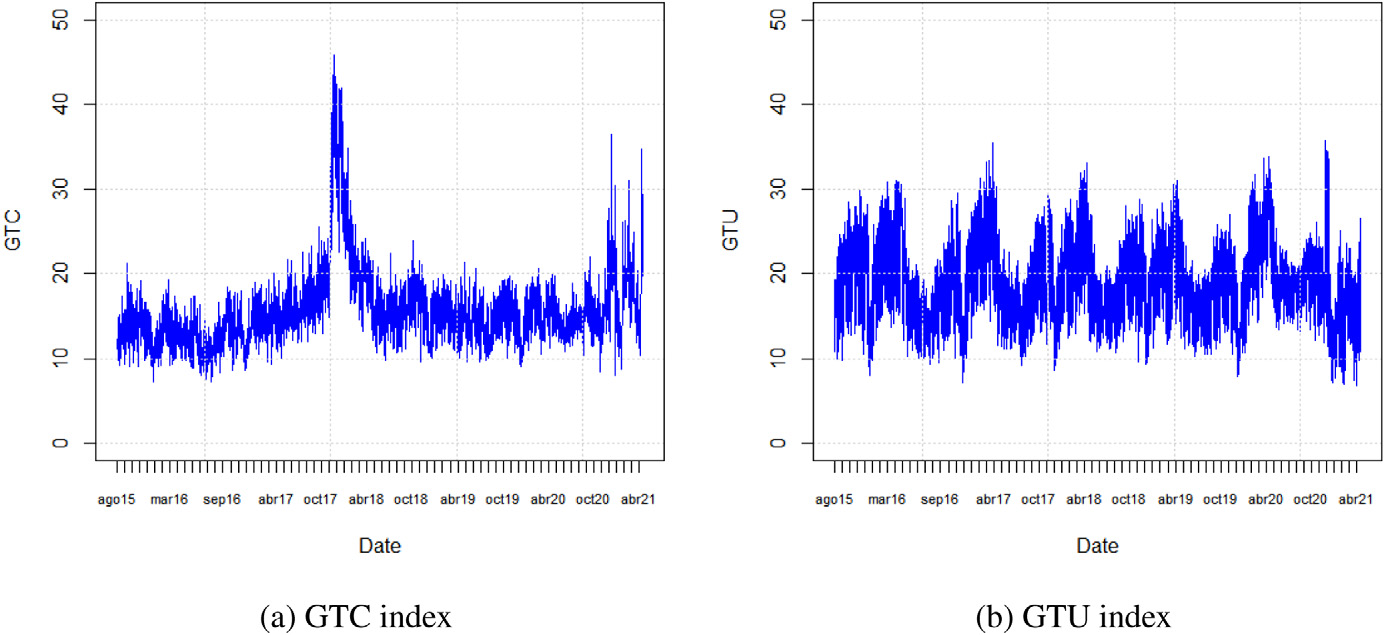
\includegraphics[width=0.9\linewidth]{gfx/m4l2_aslanidis_fig1_gtc_gtu.png}
\par\smallskip{\small \textbf{Hình 1:} Các chỉ số sự chú ý trên Google Trends: GTC và GTU (Castelnuovo and Tran, 2017).}
\end{figure}

\section{3. Phương pháp}

Chúng tôi đo lường các liên kết thông tin giữa Bitcoin và sự chú ý thị trường bằng entropy chuyển giao Shannon (transfer entropy, TE) (xem chi tiết trong Dimpfl and Peter (2013, 2018)). Entropy chuyển giao Shannon là một phương pháp phi tham số, linh hoạt, được thiết kế để khắc phục một số hạn chế của kiểm định nhân quả Granger (ví dụ như giả định tuyến tính).

Entropy chuyển giao là một thước đo dựa trên khoảng cách Kullback--Leibler của các xác suất chuyển trạng thái, cho phép không chỉ xác định hướng của luồng thông tin mà quan trọng hơn là định lượng độ mạnh của các luồng đó. Xét hai quá trình $I$ và $J$, với các phân phối xác suất biên $p(i)$ và $p(j)$, cùng phân phối xác suất đồng thời $p(i,j)$, entropy chuyển giao Shannon (TE) được định nghĩa như sau:

\begin{equation}
T_{J\to I}(k,l) = \sum_{i,j} p\left(i_{t+1}, i_t^{(k)}, j_t^{(l)}\right) \cdot \log_2\left(\frac{p\left(i_{t+1}\vert i_t^{(k)},j_t^{(l)}\right)}{p\left(i_{t+1}\vert i_t^{(k)}\right)}\right), \tag{1}
\end{equation}

trong đó $T_{J\to I}$ là thước đo lượng thông tin truyền từ $J$ đến $I$, còn $k$ và $l$ là các độ trễ (lag) được xem xét. Vì TE có thể là một ước lượng thiên lệch của lượng thông tin truyền tải, Marschinski and Kantz (2002) đề xuất một thước đo điều chỉnh, bằng cách loại bỏ phần thông tin sinh ra từ việc xáo trộn ngẫu nhiên (shuffled realization) của quá trình giải thích, như sau:

\begin{equation}
ETE_{J\to I}(k,l) = T_{J\to I}(k,l) - T_{J_{\text{shuffled}}\to I}(k,l) \tag{2}
\end{equation}

Entropy chuyển giao hiệu quả (Effective Transfer Entropy, ETE) không chỉ cho biết hướng mà còn cho biết lượng thông tin được truyền tải từ quá trình này sang quá trình kia.

Đã có tài liệu ghi nhận rằng tiền mã hóa là tài sản có độ biến động cực kỳ cao (Chaim and Laurini, 2018). Đồng thời, các lượt tìm kiếm trực tuyến có thể chịu ảnh hưởng của hành vi bầy đàn (herd behavior) (Preis et al., 2010; Bouri et al., 2019). Do đó, đáng xem xét tác động của các mức lợi suất tiền mã hóa cực đoan và các lượt tìm kiếm Google lên sự truyền tải thông tin. Ở khía cạnh này, entropy Rényi cho phép nhấn mạnh vào những phần nhất định của hàm mật độ xác suất thực nghiệm của cả hai biến.

Rényi (1970) đã phát triển một họ các thước đo thông tin thay thế cho entropy Shannon cổ điển. Một trong các thước đo đó ngày nay được biết đến với tên gọi entropy Rényi:

\begin{equation}
S_q^R(P) = \frac{1}{1-q}\log_2 \sum_{x\in X} p^q(x) \tag{3}
\end{equation}

trong đó $q$ là một tham số có thể được dùng để làm nổi bật một số phần của phân phối xác suất. Cụ thể, khi $0<q<1$, các sự kiện biên (marginal events) được nhấn mạnh nhiều hơn khi $q$ càng nhỏ trong khoảng đó. Khi $q\to 1$, ta thu lại đúng entropy Shannon.

Để ngắn gọn, chúng tôi giới thiệu độc giả tham khảo Jizba et al. (2012), Behrendt et al. (2019) để biết chi tiết về cách suy diễn entropy chuyển giao Rényi.

\section{4. Phân tích thực nghiệm}

\subsection*{4.1 Dữ liệu}

Bài báo này sử dụng dữ liệu hàng ngày về Google Trends và giá tiền mã hóa. Chúng tôi tính chỉ số Google Trends Uncertainty (GTU) của Castelnuovo and Tran (2017) cũng như chỉ số Google Trends Cryptocurrency (GTC) do chúng tôi đề xuất trong Mục 2. Dữ liệu tiền mã hóa hàng ngày được dùng để tính lợi suất logarit và độ biến động Parkinson (1980)\footnote{Mặc dù không được trình bày trong bài báo, dùng độ biến động Garman and Klass (1980) cho kết quả tương tự.}. Vì mục đích tái lập kết quả, dữ liệu sử dụng trong bài báo này được cung cấp trực tuyến cùng với bài báo. Giai đoạn khảo sát trải dài từ 07/08/2015 đến 22/04/2021, với tổng cộng 2086 quan sát.

Chúng tôi tập trung chủ yếu vào Bitcoin, vì các liên kết trên thị trường tiền mã hóa (cả về lợi suất lẫn độ biến động) đã trở nên rất mạnh trong những năm gần đây (Aslanidis et al., 2021). Như được trình bày trong tài liệu bổ sung, kết quả của chúng tôi có thể được khái quát hóa cho các đồng tiền khác như DASH, ETH, LTC và XRP.

Kết quả thực nghiệm trong mục này dùng chỉ số GTC với năm từ khóa (Tập con 3) và vẫn vững với các lựa chọn từ khóa khác. Để biết thêm chi tiết về các lựa chọn từ khóa khác nhau, xem Phụ lục A.

\subsection*{4.2 Chỉ số Google Trends Uncertainty và tiền mã hóa}

Chúng tôi khảo sát, bằng phương pháp entropy chuyển giao, sự trao đổi thông tin giữa thị trường Bitcoin và chỉ số Google Trends Uncertainty (GTU). Chúng tôi sử dụng sai phân bậc một của dữ liệu Google Trends để đảm bảo tính dừng. Bảng 1 trình bày thống kê mô tả của các biến được dùng trong phân tích.

\begin{figure}[H]
\centering
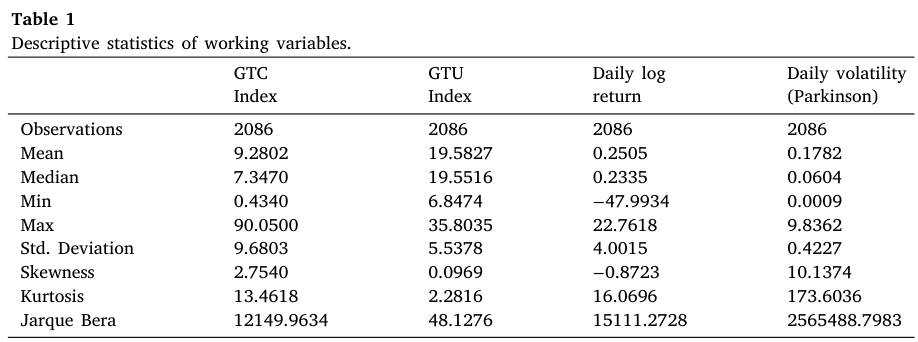
\includegraphics[width=0.8\linewidth]{gfx/m4l2_aslanidis_table1_descriptive_stats.png}
\par\smallskip{\small \textbf{Bảng 1:} Thống kê mô tả các biến được dùng trong phân tích.}
\end{figure}

Trước tiên, chúng tôi định lượng lượng thông tin truyền tải giữa GTU và Bitcoin. Bảng 2 cho thấy các luồng thông tin giữa Bitcoin và GTU không có ý nghĩa thống kê, điều này cho thấy tiền mã hóa tách biệt khỏi môi trường kinh tế vĩ mô chung. Kết quả này phù hợp với các phát hiện trước đây (Corbet et al., 2018; Aslanidis et al., 2019), vốn cho rằng các đồng tiền mã hóa lớn khá biệt lập so với các tài sản truyền thống như vàng, cổ phiếu hay trái phiếu. Phát hiện này vẫn vững đối với các lựa chọn độ trễ khác nhau, như được thể hiện trong Hình 2.

\begin{figure}[H]
\centering
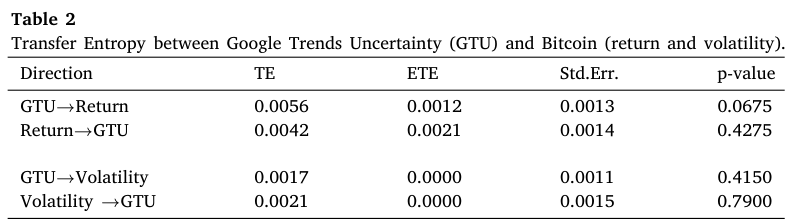
\includegraphics[width=0.8\linewidth]{gfx/m4l2_aslanidis_table2_te_gtu_bitcoin.png}
\par\smallskip{\small \textbf{Bảng 2:} Entropy chuyển giao giữa Google Trends Uncertainty (GTU) và Bitcoin (lợi suất và độ biến động).}
\end{figure}

\begin{figure}[H]
\centering
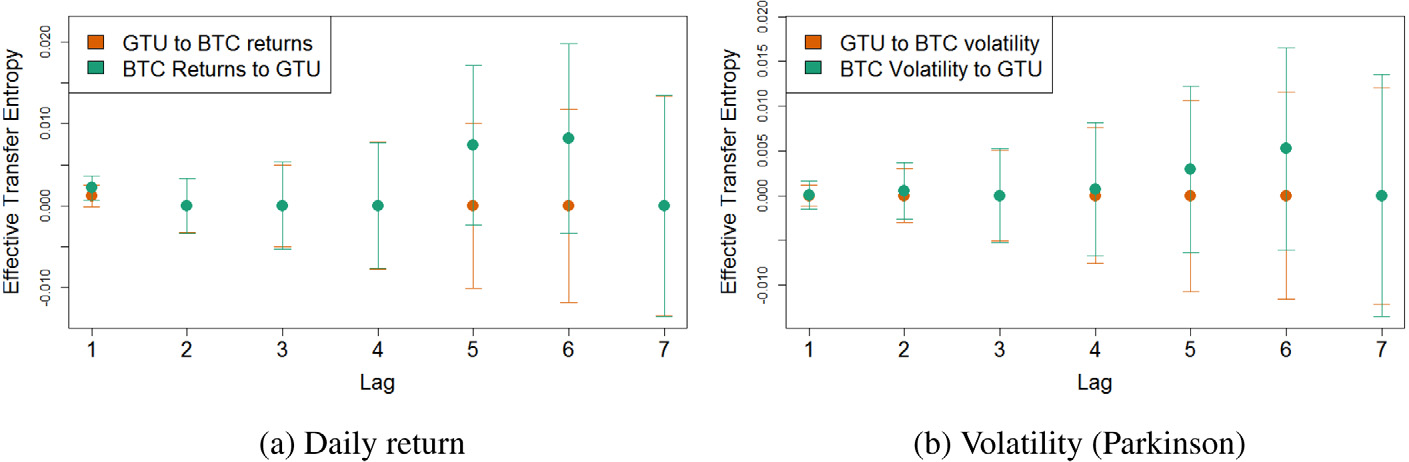
\includegraphics[width=0.9\linewidth]{gfx/m4l2_aslanidis_fig2_ete_gtu_bitcoin.png}
\par\smallskip{\small \textbf{Hình 2:} Entropy chuyển giao hiệu quả (ETE) giữa Google Trends Uncertainty (GTU) và lợi suất (a) hoặc độ biến động (b) sử dụng các độ trễ khác nhau.}
\end{figure}

\subsection*{4.3 Chỉ số Google Trends Cryptocurrency và tiền mã hóa}

Tuy nhiên, một bức tranh khác xuất hiện khi phân tích lợi suất/độ biến động của Bitcoin so với chỉ số Google Trends Cryptocurrency (GTC) được đề xuất. Bảng 3 trình bày kết quả entropy chuyển giao chỉ dùng độ trễ đầu tiên. Có thể thấy, tồn tại một luồng thông tin qua lại giữa Bitcoin và sự chú ý thị trường. Chúng tôi quan sát thấy lượng thông tin được truyền tải giữa Bitcoin và GTC là không đối xứng. Cụ thể, có nhiều thông tin rò rỉ hơn từ lợi suất (và độ biến động) của Bitcoin sang GTC so với chiều ngược lại.

\begin{figure}[H]
\centering
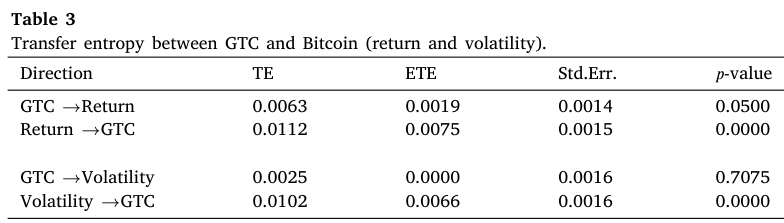
\includegraphics[width=0.8\linewidth]{gfx/m4l2_aslanidis_table3_te_gtc_bitcoin.png}
\par\smallskip{\small \textbf{Bảng 3:} Entropy chuyển giao giữa GTC và Bitcoin (lợi suất và độ biến động).}
\end{figure}

Phân tích của chúng tôi tiến thêm một bước bằng cách xem xét mối quan hệ phụ thuộc lẫn nhau, sử dụng nhiều độ trễ khác nhau của các biến. Như thể hiện trong Hình 3, lượng thông tin được truyền tải lớn hơn đối với lợi suất so với độ biến động. Hơn nữa, chúng tôi cho thấy mối quan hệ phụ thuộc lẫn nhau giữa GTC và lợi suất là hai chiều, tăng dần theo độ trễ và có ý nghĩa thống kê trong tối đa sáu ngày. Ngược lại, sự truyền tải thông tin giữa độ biến động của Bitcoin và GTC vẫn mạnh nhưng chỉ kéo dài khoảng ba đến bốn ngày, và chỉ có ý nghĩa thống kê theo chiều từ độ biến động đến GTC. Điều này hàm ý rằng tin tức được thị trường hấp thụ tương đối nhanh, mặc dù các biến động giá dường như tạo ra sự chú ý thị trường mạnh hơn trong tuần.

\begin{figure}[H]
\centering
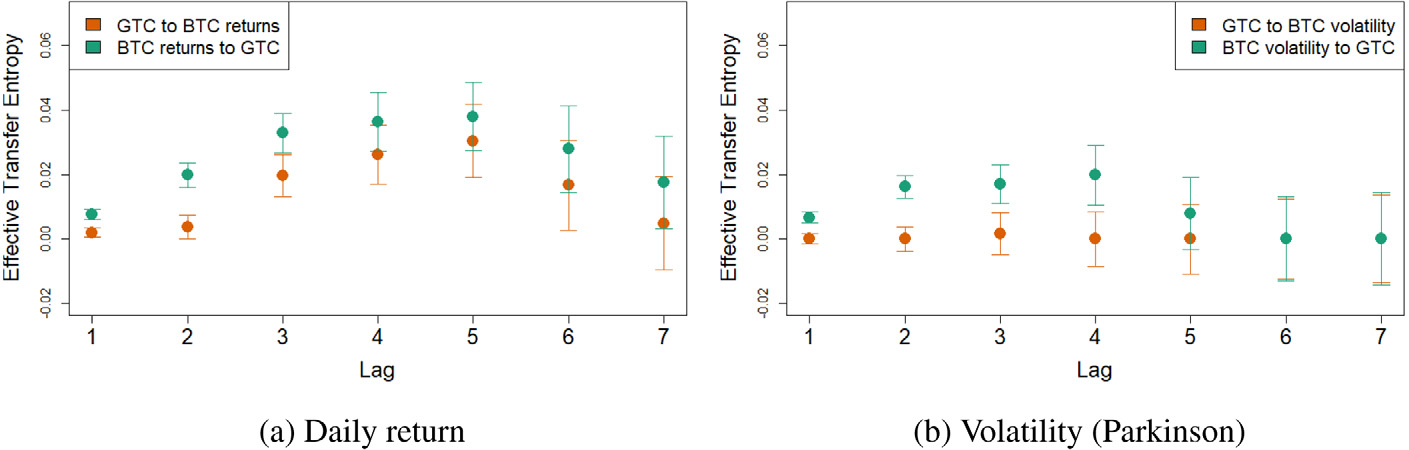
\includegraphics[width=0.9\linewidth]{gfx/m4l2_aslanidis_fig3_ete_gtc_crypto.png}
\par\smallskip{\small \textbf{Hình 3:} Entropy chuyển giao hiệu quả (ETE) giữa chỉ số Google Trends Cryptocurrency (GTC) và lợi suất (a) hoặc độ biến động (b) sử dụng các độ trễ khác nhau.}
\end{figure}

Mối liên kết hai chiều mạnh mẽ giữa Bitcoin và GTC có thể do sự chú ý ngày càng tăng của truyền thông đối với tiền mã hóa, điều khuyến khích các nhà đầu tư tìm kiếm lợi suất cao thu thập thông tin về loại tài sản tài chính mới này. Điều đó tạo ra một ``cuộc đối thoại'' giữa các lượt tìm kiếm trực tuyến và khả năng sinh lời cũng như các thước đo rủi ro của thị trường tiền mã hóa.

\subsection*{4.4 Rủi ro đuôi và truyền tải thông tin}

Entropy chuyển giao Shannon đo lường sự trao đổi thông tin giữa hai chuỗi thời gian, xem xét toàn bộ phân phối xác suất. Như đã biết, tiền mã hóa là tài sản có độ biến động rất cao và dễ xảy ra các biến động giá lớn. Đồng thời, các lượt tìm kiếm trực tuyến có thể chịu ảnh hưởng của các trào lưu nhất thời (fads), do đó thể hiện hành vi bầy đàn. Vì vậy, trong mục này chúng tôi nhằm xác định lượng thông tin nằm ở phần đuôi của phân phối lợi suất/độ biến động của Bitcoin và GTC. Entropy chuyển giao Rényi đo lường sự phụ thuộc đuôi bằng cách thiết lập giá trị của tham số $q$ trong khoảng từ 0 đến 1. Trong phân tích của mình, chúng tôi tính entropy chuyển giao Rényi cho $q=\{0.25,0.5,0.75\}$, lưu ý rằng $q$ càng nhỏ thì trọng số đặt vào phần đuôi càng lớn. Kết quả được trình bày trong Hình 4.

\begin{figure}[H]
\centering
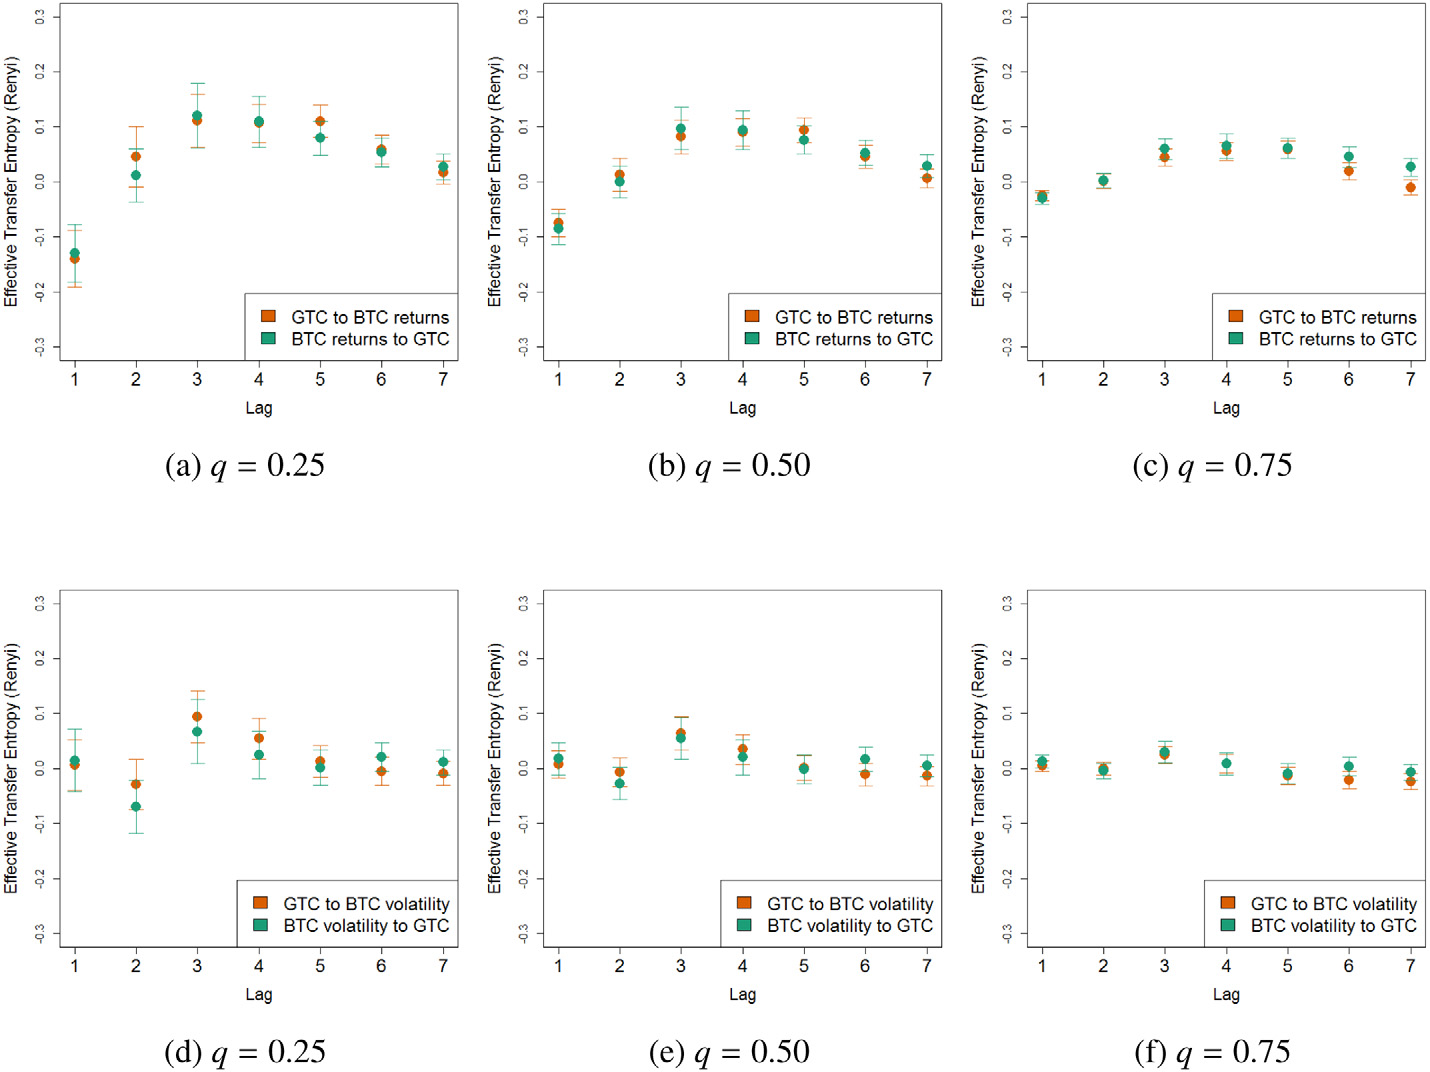
\includegraphics[width=0.95\linewidth]{gfx/m4l2_aslanidis_fig4_renyi_transfer_entropy.png}
\par\smallskip{\small \textbf{Hình 4:} Entropy chuyển giao Rényi (với các giá trị $q$ khác nhau) giữa chỉ số Google Trends Cryptocurrency (GTC) và lợi suất/độ biến động của Bitcoin (BTC) sử dụng các độ trễ khác nhau.}
\end{figure}

Phù hợp với các kết quả trước đó, luồng thông tin giữa chỉ số GTC và lợi suất Bitcoin lớn hơn so với giữa chỉ số GTC và độ biến động của Bitcoin. Tương tự, hình dạng của mối quan hệ này giữ nguyên qua các độ trễ khác nhau. Lượng thông tin truyền tải giữa GTC và lợi suất có ý nghĩa thống kê trong tối đa sáu ngày. Tuy nhiên, chúng tôi phát hiện một khác biệt đáng kể về độ lớn của luồng thông tin. Cụ thể, khi các sự kiện cực đoan được đặt trọng số cao, lượng thông tin được truyền tải lớn hơn, đạt cực đại sau ba ngày.

Đối với độ biến động, kết quả nhìn chung phù hợp với kết quả thu được khi sử dụng entropy Shannon. Sự truyền tải thông tin giữa GTC và độ biến động của Bitcoin rất ít. Tuy nhiên, khi tập trung vào các sự kiện cực đoan ($q=0.25$), vẫn có một phần thông tin được truyền tải, nhưng chỉ trong tối đa ba ngày.

\section{5. Kết luận}

Chúng tôi xác nhận rằng thị trường tiền mã hóa khá tách biệt khỏi môi trường kinh tế vĩ mô chung như được đo lường gián tiếp bằng các chỉ số Google Trends Uncertainty, chẳng hạn như chỉ số của Castelnuovo and Tran (2017). Thay vào đó, chỉ số Google Trends Cryptocurrency mà chúng tôi đề xuất truyền tải các luồng thông tin quan trọng đến (và nhận phản hồi từ) thị trường tiền mã hóa.

Chúng tôi cho thấy rằng sự truyền tải thông tin giữa Google Trends và lợi suất hàng ngày là hai chiều và kéo dài đến sáu ngày. Hơn nữa, các luồng thông tin từ độ biến động của Bitcoin đến chỉ số chú ý trên Google Trends được phát hiện là lớn hơn so với chiều ngược lại. Bài báo này cũng ghi nhận sự phụ thuộc đuôi đáng kể, cụ thể là giữa chỉ số Google Trends Cryptocurrency và lợi suất Bitcoin, phản ánh tầm quan trọng của các sự kiện cực đoan đối với những người tham gia thị trường.

Kết quả của chúng tôi vững đối với các cách kết hợp khác nhau của chỉ số Google Trends Cryptocurrency. Trên thực tế, chỉ cần năm từ khóa là đủ để nắm bắt sự chú ý thị trường, điều này phản ánh một chiến lược tìm kiếm không quá phức tạp của nhà đầu tư. Hơn nữa, các phát hiện của chúng tôi không chỉ đặc thù cho riêng Bitcoin, mà còn áp dụng được cho các đồng tiền mã hóa lớn khác như Dash, Ethereum, Litecoin và Ripple.

Gần đây, thị trường tiền mã hóa đã thu hút sự chú ý đáng kể từ các ngân hàng đầu tư (ví dụ: Morgan Stanley, Goldman Sachs), các nhà đầu tư mạo hiểm, các cơ quan quản lý (việc phê duyệt các quỹ ETF Bitcoin tại Canada) và các nhà hoạch định chính sách (quyết định của El Salvador công nhận Bitcoin và Ethereum là phương tiện thanh toán hợp pháp), cho thấy sự quan tâm của các định chế đang ngày càng gia tăng. Hơn nữa, Bank for International Settlements (2021) đã khởi động một quá trình tham vấn nhằm thu thập ý kiến về khả năng các ngân hàng thương mại nắm giữ Bitcoin và các tài sản kỹ thuật số khác. Mặc dù nghiên cứu của chúng tôi không phát hiện mối quan hệ đáng kể nào giữa Bitcoin và nền kinh tế vĩ mô nói chung, quá trình thể chế hóa tiền mã hóa có thể khiến chúng dần thâm nhập vào hệ sinh thái tài chính truyền thống. Nhìn chung, nghiên cứu của chúng tôi mang lại những hàm ý quan trọng cho việc quản lý quỹ đầu tư và hoạch định chính sách, vì nó cung cấp thông tin quan trọng để thiết kế và tái cân bằng danh mục đầu tư.

\section{Tuyên bố đóng góp tác giả (CRediT)}

\textbf{Nektarios Aslanidis:} Hình thành ý tưởng, Phương pháp luận, Viết (rà soát \& biên tập), Phân tích chính thức. \textbf{Aurelio F. Bariviera:} Hình thành ý tưởng, Phương pháp luận, Viết (rà soát \& biên tập), Phần mềm, Phân tích chính thức. \textbf{Óscar G. López:} Viết (rà soát \& biên tập), Phần mềm.

\section{Lời cảm ơn}

Nektarios Aslanidis ghi nhận sự hỗ trợ của Chính phủ Tây Ban Nha thông qua dự án PID2019-105982GB-I00. Óscar G. López ghi nhận sự hỗ trợ từ học bổng nghiên cứu của Văn phòng Quốc vụ khanh về Giáo dục và Đào tạo nghề (Secretary of State for Education and Vocational Training, Tây Ban Nha), năm 2020, mã COLAB 00559.

\section{Phụ lục A. Bộ từ khóa xây dựng Chỉ số Chú ý Google Trends Cryptocurrency (GTC)}

Xem Bảng A.4. Bảng dưới đây liệt kê các bộ từ khóa (được giữ nguyên tiếng Anh vì đây là các từ khóa tìm kiếm thực tế dùng để truy vấn Google Trends).

\textbf{Bộ đầy đủ (38 từ khóa):} AES256, altcoin, anonymity, Bitcoin, block producer, blockchain, BTC, coin, consensus, crypto, crypto crash, cryptocurrency, cryptography, digital assets, distributed ledger, ethereum, hard fork, hash, hashing, ICO, miner, minted, public key, ripple, satoshi, soft fork, stablecoin, tether, token, virtual currency, Mount Gox, Mt Gox, Mt. Gox, private key, Proof of Authority, Proof of Burn, Proof of Stake, Proof of Work.

\textbf{Tập con 1 (Subset 1):} anonymity, Bitcoin, blockchain, BTC, coin, consensus, crypto, cryptocurrency, ICO, cryptography, ethereum, hash, miner, minted, public key, ripple, satoshi, stablecoin, token, private key, Proof of Work.

\textbf{Tập con 2 (Subset 2):} Bitcoin, blockchain, BTC, crypto, cryptocurrency, cryptography, ethereum, ripple, satoshi, tether.

\textbf{Tập con 3 (Subset 3):} Bitcoin, blockchain, BTC, crypto, cryptocurrency.

\par\smallskip{\small \textbf{Bảng A.4:} Các bộ từ khóa được xem xét trong Chỉ số Chú ý Google Trends Cryptocurrency (GTC).}

\section{Phụ lục B. Dữ liệu bổ sung}

Tài liệu bổ sung liên quan đến bài báo này có thể được tìm thấy trực tuyến tại \url{https://doi.org/10.1016/j.frl.2021.102654}.

% [Đã lược bỏ danh mục Tài liệu tham khảo gốc (tiếng Anh, trích dẫn của tác giả bài gốc) để giảm dung lượng chương; không ảnh hưởng nội dung học thuật chính.]
